\documentclass[10pt,letterpaper]{article}

\usepackage{amsmath}

\usepackage[T1]{fontenc} 
\usepackage[utf8x]{inputenc}
\usepackage[spanish]{babel}
\usepackage{graphicx}% Include figure files

\usepackage{fancyvrb,xcolor}
\usepackage{upquote,textcomp}

%%% Margins
\oddsidemargin=-1.00cm
\textwidth=18.0cm
\topmargin=-2.54cm
\headheight=0cm
\headsep=2cm
\textheight=23.8cm

\makeatletter
\renewcommand\section{\@startsection{section}{1}{-15pt}{20pt}{10pt}{\textsc}}
\makeatother

\makeatletter
\renewcommand\subsection{\@startsection{subsection}{2}{0pt}{0pt}{0pt}{\textit}}
\makeatother

\usepackage{hyperref} % for urls


% Default fixed font does not support bold face
\DeclareFixedFont{\ttb}{T1}{txtt}{bx}{n}{8} % for bold
\DeclareFixedFont{\ttm}{T1}{txtt}{m}{n}{8}  % for normal

% Custom colors
\usepackage{color}
\definecolor{deepblue}{rgb}{0,0,0.5}
\definecolor{deepred}{rgb}{0.6,0,0}
\definecolor{deepgreen}{rgb}{0,0.5,0}
\definecolor{deepgray}{rgb}{0.5,0.5,0.5}

\usepackage{listings}

\lstdefinestyle{myCustomPythonStyle}{
	language=Python,
	basicstyle=\linespread{1}\small,
	otherkeywords={self},             % Add keywords here
	keywordstyle=\ttb\color{deepblue},
	emph={MyClass,__init__},          % Custom highlighting
	emphstyle=\ttm\color{deepred},    % Custom highlighting style
	commentstyle=\ttm\color{deepgray},
	stringstyle=\color{deepgreen},
	frame=tb,                         % Any extra options here
	showstringspaces=false,
	columns=fullflexible,
	keepspaces=true,
	literate={-}{-}1,				% To avoid problems with hyphen -
}



\makeatletter 
  \renewcommand\verbatim@font{\normalfont\ttfamily\color{blue}}
\makeatother


\begin{document}
% To fix ' no curve quotation mark
\newcommand\upquote[1]{\textquotesingle#1\textquotesingle}



\begin{tabular}{p{1.3in}p{6in}}
\begin{flushleft}
\noindent 
\includegraphics[bb = 2.5cm 0cm 10.29cm 9.78cm,scale=0.2]{./figures/escudoUnicacuaSolo.eps}
\end{flushleft} &
\normalsize \vspace{0.6cm}
\textsc{Universidad del Cauca}

\textsc{Facultad de Ingeniería Electrónica y Telecomunicaciones}

%\textsc{Maestría en Ingeniería Telemática}
\textsc{Programa de Ingeniería Electrónica y Telecomunicaciones}

%\textsc{Desarrollo de aplicaciones para plataformas ubicuas}

\textsc{ScientoPy, Installation and User Manual}

\end{tabular}
\begin{tabbing}
\hspace{3cm} \= \hspace{5.3cm} \= \hspace{6cm} \kill
\textbf{By}: \> Juan Pablo Ruiz Rosero			\> \texttt{jpabloruiz@unicauca.edu.co} \\
\end{tabbing}

\section{Installation}

\begin{enumerate}
\item Download and install the last version of Python 2.7 (for example Python 2.7.14) from: \\ \url{https://www.python.org/downloads/}
\item Install the matplotlib library for Python the automatic installation tool \textbf{pip}. From Windows, enter in the command line (Windows + R, cmd, and Enter), go to the folder \verb|C:\Python27\Scripts|, and run the installation script:
\begin{verbatim}
cd C:\Python27\Scripts
pip install matplotlib
\end{verbatim}
\end{enumerate}


\section{Download the bibliometric dataset}
This section describes how to download the proper dataset from Scopus and WoS. Define a search criteria, it will be used for Scopus and WoS. For this guide we are using: "Internet of thing"  AND  "Gateway" 

\subsection{Download the dataset from Scopus}
\begin{enumerate}
\item Make your search with the defined search criteria for Article title, Abstract, Keywords. 
\item Select all the results and click on Export:
	\begin{center}
		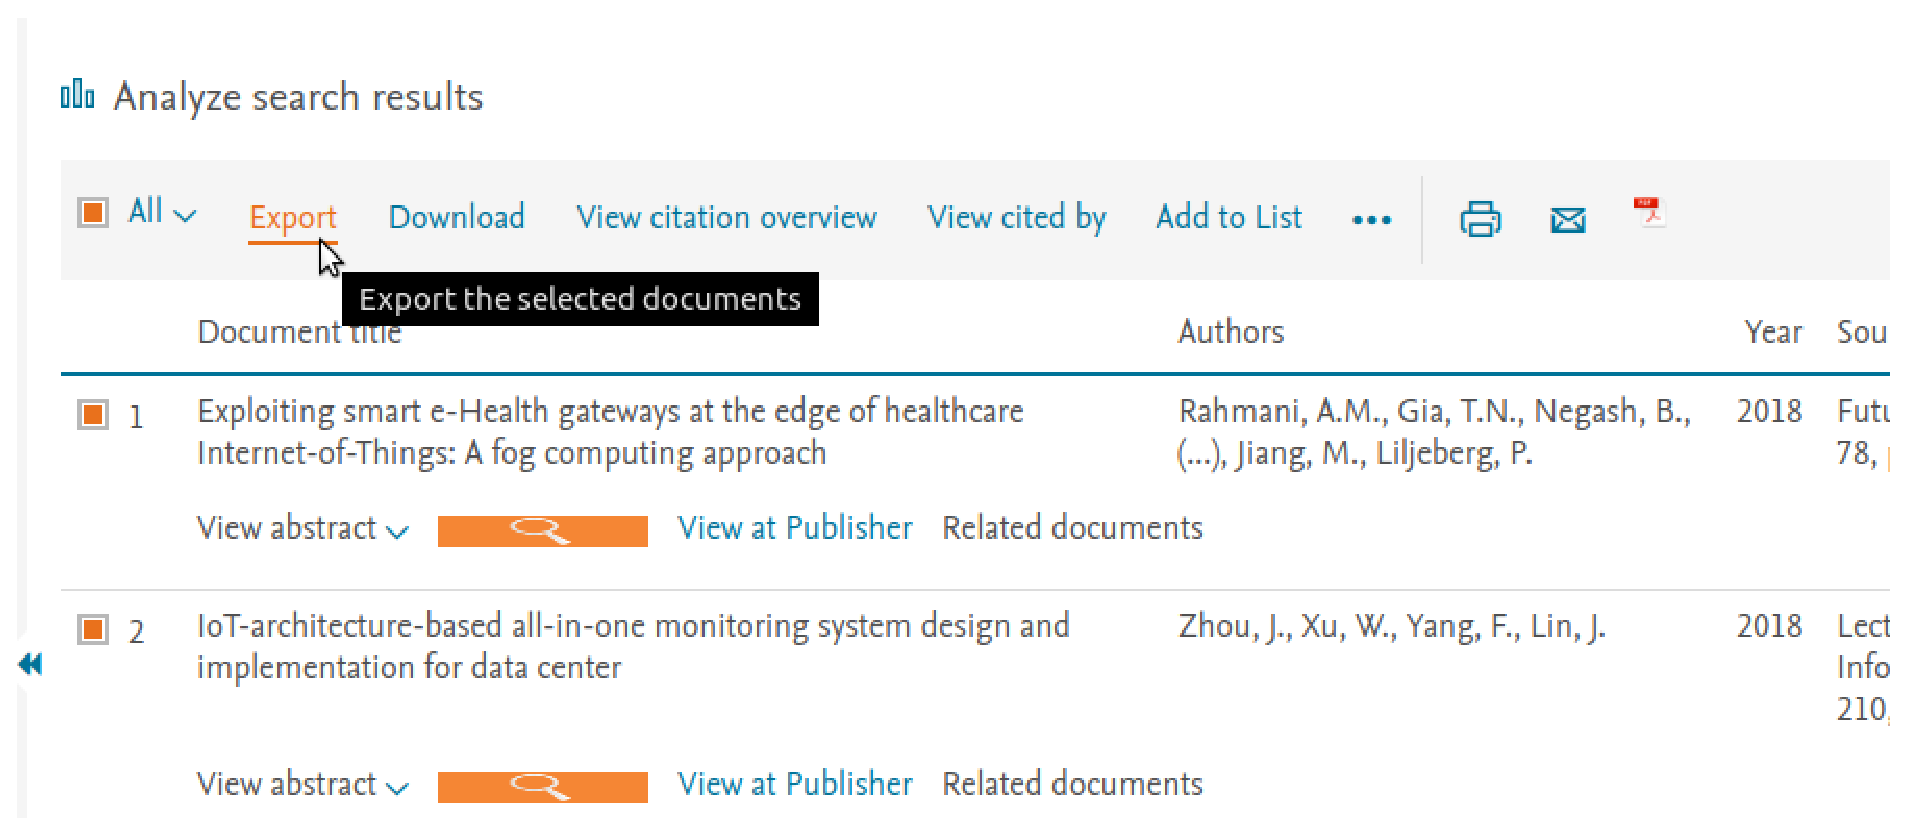
\includegraphics[scale=0.33]{./figures/scopus1.eps}
	\end{center}

\item Select as method of export \textbf{CSV (Excel)}, and select the Customize export \textbf{Citation information, Bibliographical information, Abstract and Keywords}, then click on Export: 
	\begin{center}
		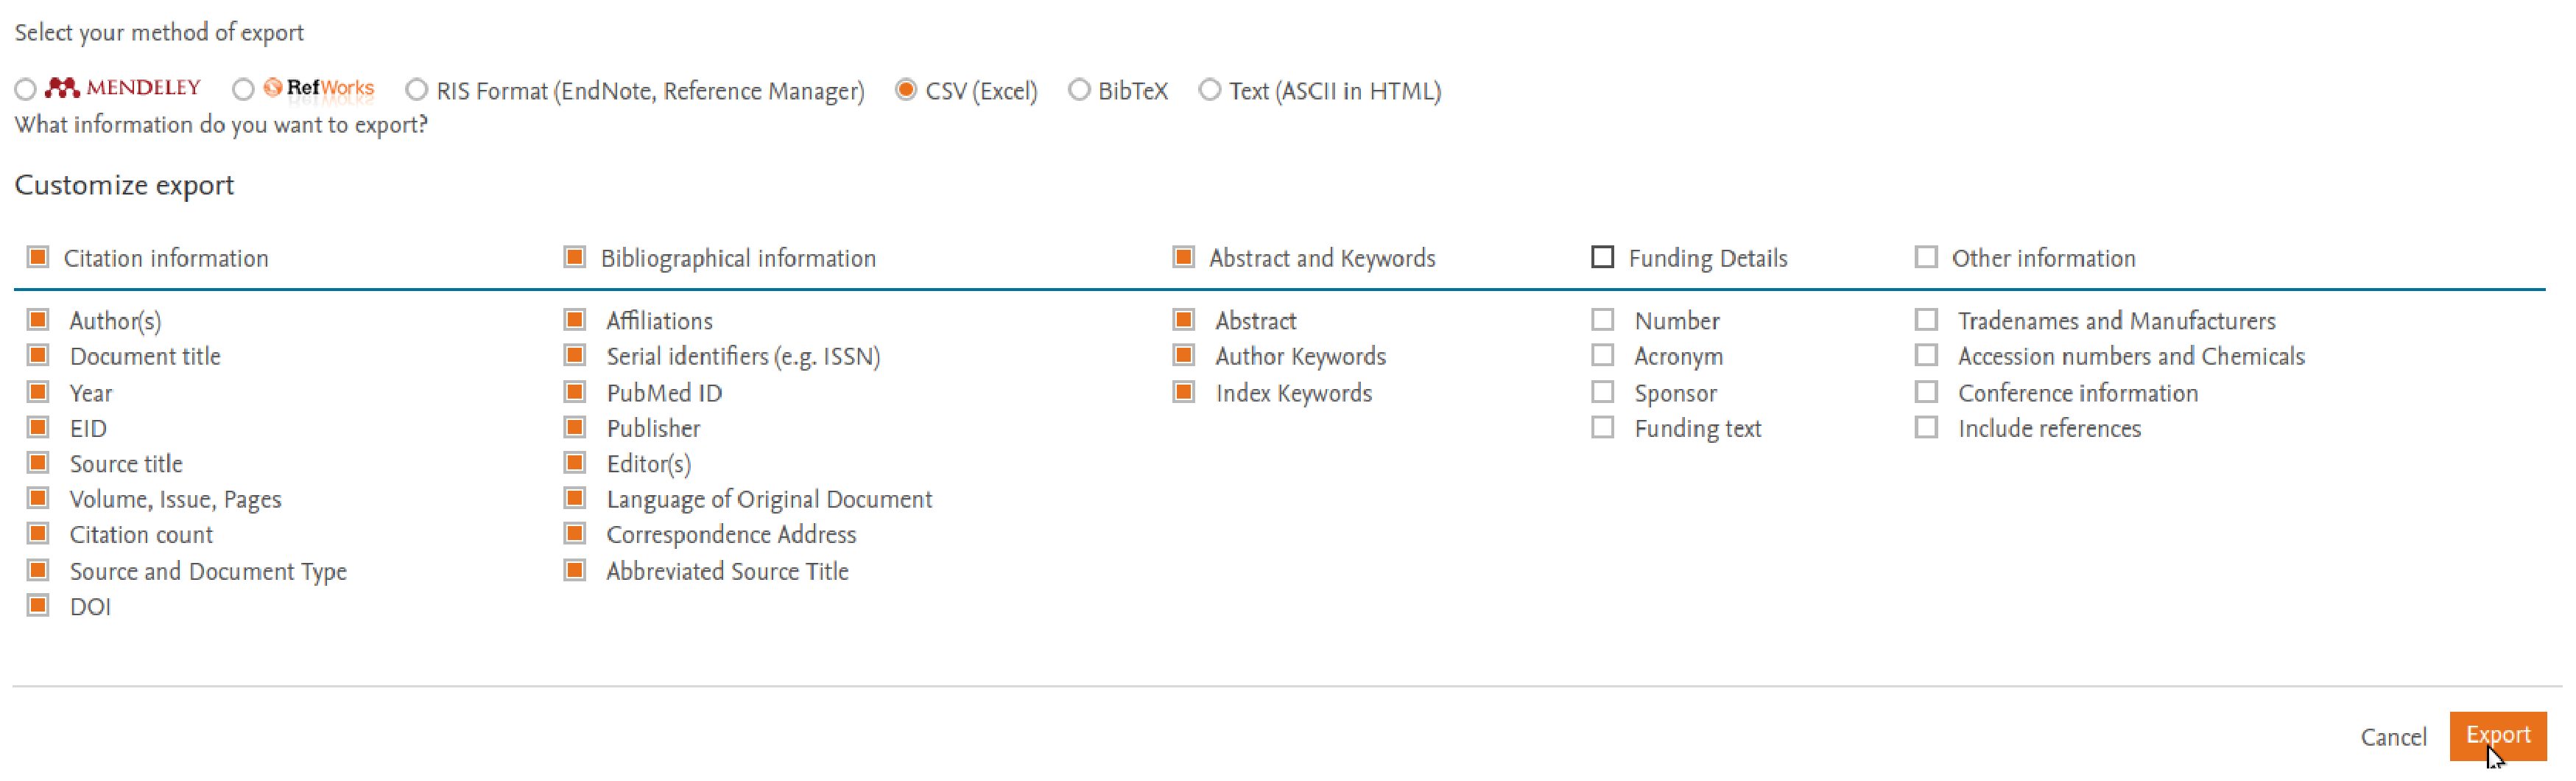
\includegraphics[scale=0.3]{./figures/scopus2.eps}
	\end{center}

\item Save the file on the folder \verb|/ScientoPy/dataIn|
\end{enumerate}


\subsection{Download the dataset from WoS}
\begin{enumerate}
\item Make your search with the defined search criteria for Topic. 
\item Select \textbf{Save in Other File Formats}
	\begin{center}
		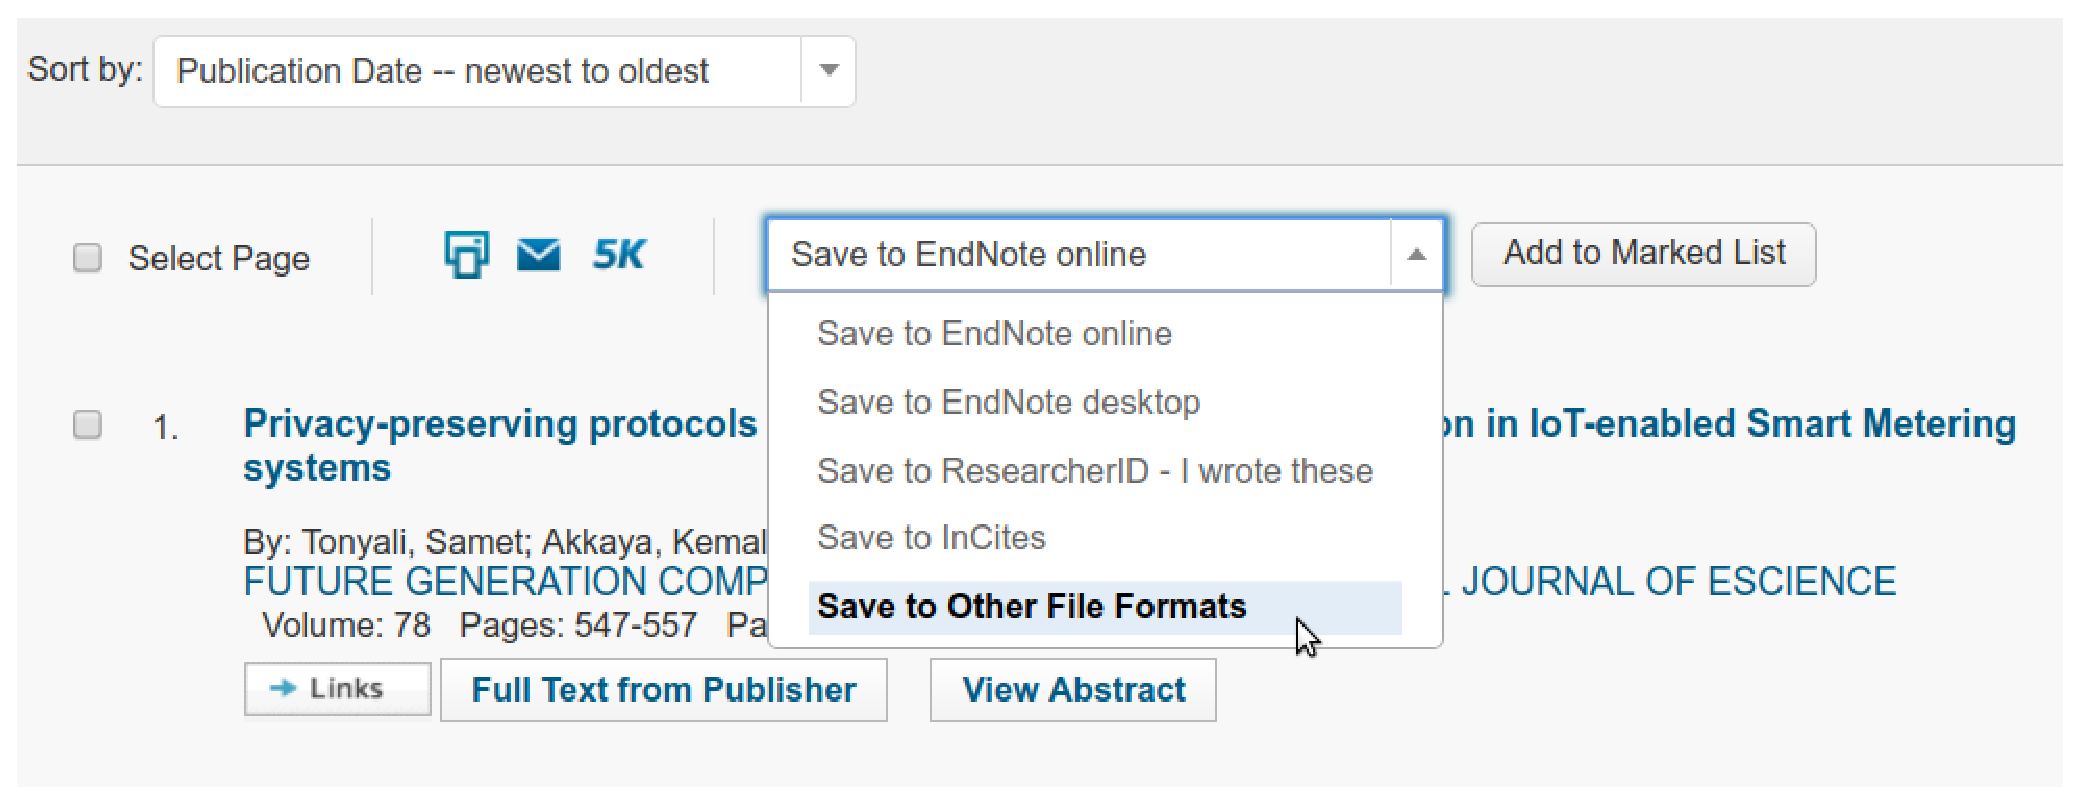
\includegraphics[scale=0.33]{./figures/wos1.eps}
	\end{center}

\item Select the number of records to download, on Record Contented select \textbf{Full Record and Cited References}, on File Format select \textbf{Tab-delimited (Win, UTF-8)}, and click on Send.
	\begin{center}
		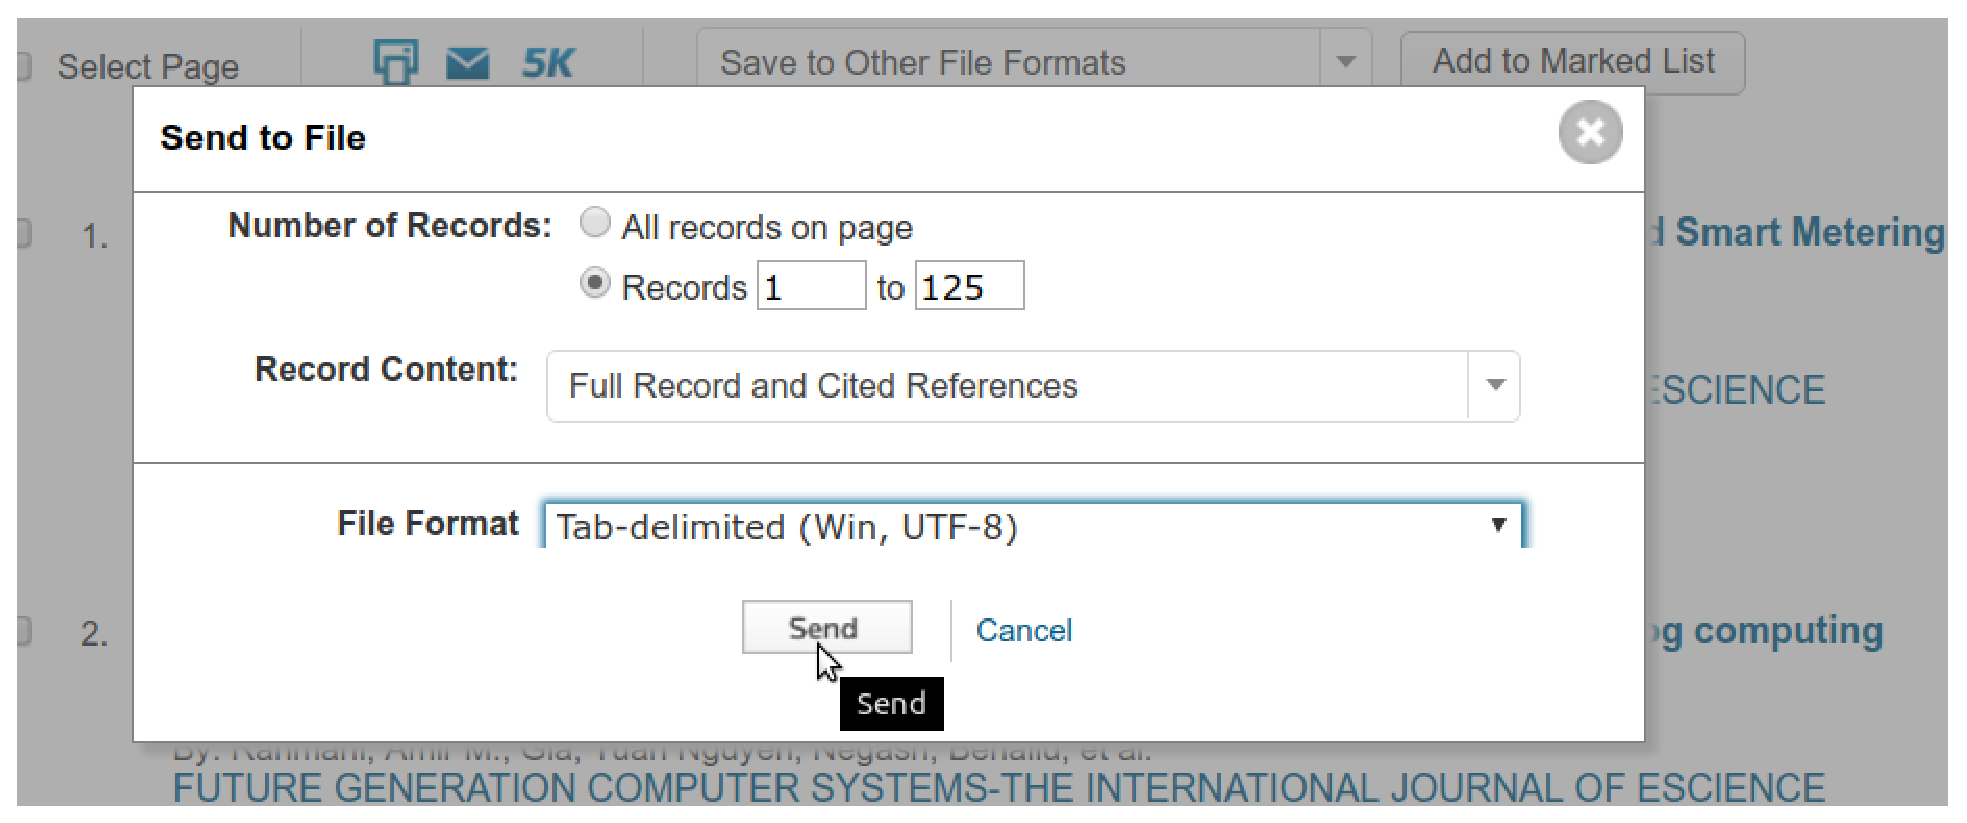
\includegraphics[scale=0.33]{./figures/wos2.eps}
	\end{center}

\item Save the file on the folder \verb|/ScientoPy/dataIn|
\end{enumerate}

\section{Running the ScientoPy scripts}

\subsection{Pre-processing}

First we need to pre-process the downloaded data. This pre process joint all the downloaded files from one folder to a single file. Also, this process remove the duplicated files. To pre-process the example dataset run this command inside ScientoPy folder: 
\begin{verbatim}
python preProcess.py dataInExample
\end{verbatim}
On the folder \verb|ScientoPy/dataPre| you will find the following files: 
\begin{itemize}
\item \textbf{papersPreprocessed.csv:} this file contains the information of all papers after the pre process. This will used by the others scripts as the input data. 
\item \textbf{PreprocessedBrief.csv:} this file briefs the pre-process statics results, such as duplicated papers removed, types of documents and others. 
\end{itemize}

To find more options of the pre-processing script you can run:
\begin{verbatim}
python preProcess.py -h
\end{verbatim}

\subsection{Extract the top topics}

With this script you can extract the top topics of a selected criterion. The ScientoPy script criteria are:

\begin{itemize}
\item authors
\item source
\item subject 
\item authorKeywords 
\item indexKeywords 
\item documentType 
\item dataBase 
\item country
\end{itemize}

For example, to find the top author's keywords you can run this script: 

\begin{verbatim}
python topResults.py authorKeywords
\end{verbatim}

This will generate a list with the top 10 topics on the criterion author's keywords, with the number of documents per topic, and the h-index associated to each one. Also, this script will graph the evolution of each topic across the year, and will save the quantitative results on the folder \verb|ScientoPy/results|. 

This script have more options like, save the plot on a file, or increase the number of topic results. For more information you can run:

\begin{verbatim}
python topResults.py -h
\end{verbatim}

\subsection{Analyze pre defined topics inside a criterion}

If you want to make an analysis of pre defined topics, such as the number of papers evolution of two countries, you should use the \verb|analizeTopic.py| script: 

\begin{verbatim}
python analizeTopic.py country -t "United States; Brazil"
\end{verbatim}

You can analyze any topic in any criterion. Put the topics on the \verb|-t| argument. Divide the topics with the \verb|;|. Also, you can integrate two or more topics in one, by dividing it with \verb|,|. This is very useful for abbreviations and plural singulars, for example: 
\begin{verbatim}
python analizeTopic.py authorKeywords -t \
"WSN, Wireless sensor network, Wireless sensor networks; RFID, RADIO FREQUENCY IDENTIFICATION"
\end{verbatim}

This script have more options like, save the plot on a file, or others. For more information you can run:

\begin{verbatim}
python analizeTopic.py -h
\end{verbatim}


\end{document}  